\documentclass[11pt]{beamer}
\usepackage[utf8]{inputenc}
\usepackage[english]{babel}
\usepackage[titletoc]{appendix}
\usepackage{sjlatex/stata}
\usepackage{float}

\usepackage[nottoc,notlot,notlof]{tocbibind}
\usepackage{bbm}
\usepackage{xifthen}
\usepackage{amsmath}
\usepackage{amsfonts}
\usepackage{natbib}
\usepackage{amsthm}
\usepackage{appendix}
\usepackage[ruled,vlined]{algorithm2e}
\usepackage{graphicx}
\usepackage{epstopdf}

\usepackage{geometry}
\setlength{\headheight}{14pt}
\setlength{\topmargin}{0pt}
\setlength{\textheight}{620pt}
\setlength{\footskip}{10pt}
\setlength{\oddsidemargin}{0pt}
\setlength{\evensidemargin}{0pt}
\geometry{
  top=15mm,
  left=15mm,
}

\usepackage{hyperref}
\hypersetup{
colorlinks,
citecolor=black,
filecolor=black,
linkcolor=black,
urlcolor=black
}


\usepackage{setspace}
\onehalfspacing

\usepackage{enumitem}

\newtheorem{defi}{DEFINITION}
\newtheorem{lemma}{LEMMA}
\newtheorem{assumption}{ASSUMPTION}
\newtheorem{theorem}{THEOREM}
\newtheorem{remark}{REMARK}
\newtheorem{prop}{PROPOSITION}

\newcommand{\ivqreg}{{\tt ivqregress}}
\newcommand{\ivqregiqr}{{\tt ivqregress iqr}}
\newcommand{\ivqregsee}{{\tt ivqregress smooth}}
\newcommand{\I}{\mathbbm{1}}
\newcommand{\Is}{\widetilde{\mathbbm{1}}}
\newcommand{\E}{\mathbf{E}}
\newcommand{\hsee}{h^*_{SEE}}
\DeclareMathOperator*{\argmax}{arg\,max}
\DeclareMathOperator*{\argmin}{arg\,min}

\newcommand{\Xb}{\mathbf{X}}
\newcommand{\Db}{\mathbf{D}}
\newcommand{\Zb}{\mathbf{Z}}
\newcommand{\UD}{U_\Db}
\newcommand{\Wb}{\mathbf{W}}
\newcommand{\xb}{\mathbf{x}}
\newcommand{\db}{\mathbf{d}}
\newcommand{\zb}{\mathbf{z}}
\newcommand{\Ud}{U_\db}
\newcommand{\Yd}{Y_\db}
\newcommand{\bb}{\mathbf{b}}
\newcommand{\Jb}{\mathbf{J}}
\newcommand{\Sb}{\mathbf{S}}
\newcommand{\Ab}{\mathbf{A}}
\newcommand{\Rb}{\mathbf{R}}
\newcommand{\rb}{\mathbf{r}}
\newcommand{\vb}{\mathbf{v}}
\newcommand{\gb}{\mathbf{g}}
\newcommand{\cb}{\mathbf{c}}
\newcommand{\gammab}{\boldsymbol{\gamma}}
\newcommand{\betab}{\boldsymbol{\beta}}
\newcommand{\alphab}{\boldsymbol{\alpha}}
\newcommand{\thetab}{\boldsymbol{\theta}}
\newcommand{\Psib}{\boldsymbol{\Psi}}
\newcommand{\Phib}{\boldsymbol{\Phi}}
\newcommand{\Omegab}{\boldsymbol{\Omega}}
\newcommand{\Lambdab}{\boldsymbol{\Lambda}}


\newcommand{\dil}[1]{{\color{red}#1}}


\title{Instrumental Variables Quantile Regression in Stata}
\author{Di Liu}
\institute{StataCorp}
\date{}

\begin{document}
\maketitle

%------------------------------------------------------------------------------
\section{Motivation and Overview}

\begin{frame}
  \frametitle{Motivation: Quantile regression with endogneity}
%------------------------------------------------------------------------------
  \begin{itemize}
    \setlength\itemsep{1em}

    \item \myred{Beyond the mean:} How would the participation in a 401(k)
      affect the lower-level, median, and upper-level conditional quantile of
      net wealth? 

    \item \myblue{Endogeneity:} The participation in a 401(k) may depend on
      the unobservable saving preference that would also affect net wealth
      growth.

    \item \myblue{IV:} Conditional on income and other covariates, the
      eligibility of 401(k) can serve as an instrument \citep{Poterba1995}.
  \end{itemize}

  \begin{align*}
    \text{\Large \myblue{Endogeneity}} & 
  	+ \text{\Large \myred{Quantile regression}} \\
  \Big \Uparrow \\
 \text{\Large \myblue{IV}}
\end{align*}
\end{frame}

%------------------------------------------------------------------------------
\begin{frame}
  \frametitle{When is estimating $E(y|x)$ not adaquate?}
%------------------------------------------------------------------------------
Consider $E(y|x) = \beta_0 + \beta_1 x_1$, then
$$\beta_1 = E(y| x = a+1) - E(y | x=a)$$

\vskip 0.4cm
{\bf Two senarios}
\begin{enumerate}
  \item The conditional density $f(y | x=a+1)$ is \myblue{only location-shifted}
    relative to $f(y | x=a)$. Then 
    \myblue{$$\beta_1 = Q(y|x=a+1, \tau) - Q(y|x=a, \tau)$$}

  \item The conditional density $f(y | x=a+1)$ is \myred{both location-shifted
  and scaled} relative to $f(y | x=a)$. Then 
    \myred{$$\beta_1 \neq Q(y|x=a+1, \tau) - Q(y|x=a, \tau)$$}


\end{enumerate}


\end{frame}

%------------------------------------------------------------------------------
\begin{frame}
  \frametitle{Beyond the mean}
%------------------------------------------------------------------------------
  \begin{center}
	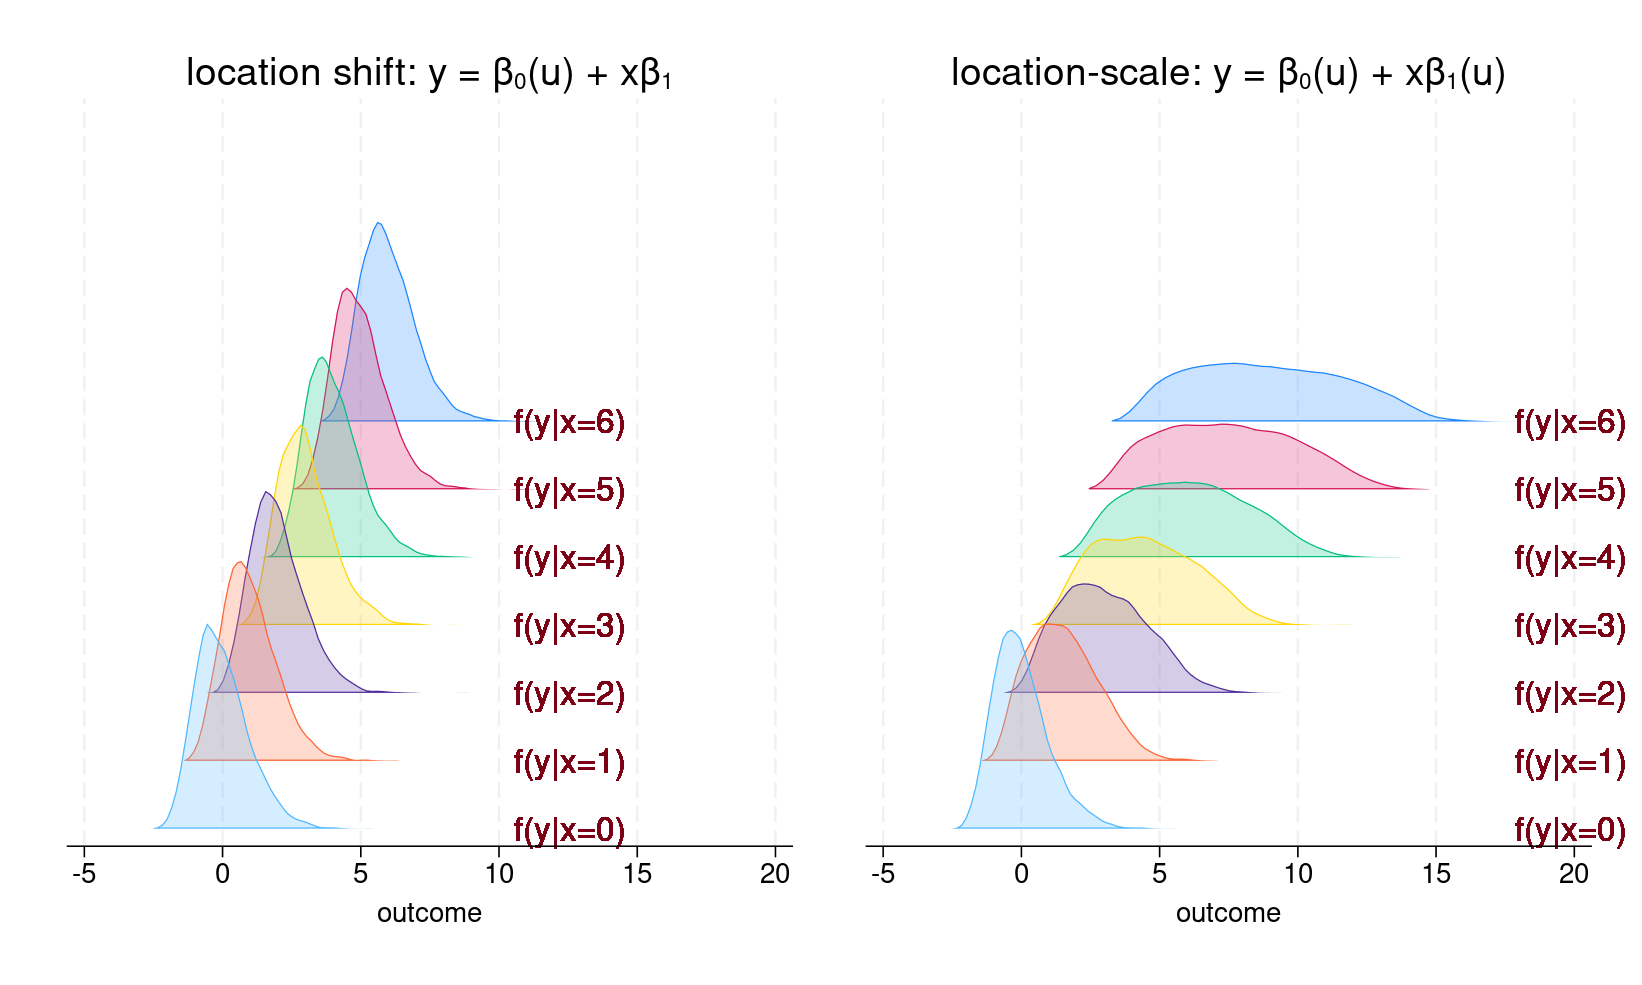
\includegraphics[scale=0.2]{eps/beyondm}
  \end{center}
\end{frame}

%------------------------------------------------------------------------------
\begin{frame}
  \frametitle{Overview of {\tt ivqregress} toolbox (I) } 
%------------------------------------------------------------------------------
  We provide a suite of commands to \myred{estimate}, \myred{visualize},
  \myred{make the inference}, and \myred{diagnose} the \myblue{linear IV
  quantile regression} models (IVQR).

  \vskip 1cm

  \begin{itemize}

    \setlength\itemsep{1.5em}

    \item \myred{Estimation}

      \begin{itemize}
    
	\setlength\itemsep{1.5em}

	\item \myblue{\tt ivqregress iqr} implements the \myred{I}nverse
	  \myred{Q}uantile \myred{R}egression estimator in
	  \cite{chernozhukov2006}.

	\item \myblue{\tt ivqregress smooth} implements the \myred{S}moothed
	  \myred{E}stimating \myred{E}quation estimator in \cite{kaplan2017}.
      \end{itemize}

  \end{itemize}
\end{frame}

%------------------------------------------------------------------------------
\begin{frame}
  \frametitle{Overview of {\tt ivqregress} toolbox (II) } 
%------------------------------------------------------------------------------
  \begin{itemize}

    \setlength\itemsep{1.5em}

    \item \myred{Visualization}
      \begin{itemize}
	\item \myblue{\tt estat coefplot} shows how the treatment effects
	  vary at different conditional quantiles of outcome.
      \end{itemize}

    \item \myred{Inference}
      \begin{itemize}
	\item \myblue{\tt estat endogeffects} tests the hypothesis regarding the
	  quantile process.

	\item \myblue{\tt estat dualci} provides the confidence interval robust
	  to weak instruments (only after {\tt ivqregress iqr}).
      \end{itemize}

     \item \myred{Diagnosis}
       \begin{itemize}
	 \item \myblue{\tt estat waldplot} helps to visually inspect the
	   convergence of the IQR estimator (only after {\tt ivqregress iqr}).
	\end{itemize}

 	\item \myred{Standard post-estimation}
       \begin{itemize}
	   \item {\tt test}, {\tt testnl}, {\tt predict}, {\tt margins}, \ldots
	\end{itemize}

  \end{itemize}
\end{frame}

%------------------------------------------------------------------------------
\section{Model and Example}
\begin{frame}
  \frametitle{Model}
%------------------------------------------------------------------------------
We can write the IV quantile regression model as a random-coefficients model
\citep{chernozhukov2008}.

\begin{align}
  y &= \myred{\db'} \myblue{\alphab(u)} + \xb' \myblue{\betab(u)} &\quad u|\xb,
  \myred{\zb} \sim
  Uniform(0,1) \\
  \db & = \delta(\xb, \myred{\zb}, v) &\quad \myred{v \text{ statistically
  depends on } u}\\
 \tau &\rightarrow \db' \alphab(\tau) + \xb' \betab(\tau) &\quad \text{ is
   strictly increasing}
\end{align}

{\bf Objective}:
\begin{itemize}
    \setlength\itemsep{1em}
    \item The coefficients (\myblue{$\alphab(\tau)$} or \myblue{$\betab(\tau)$})
      summarize the \myblue{marginal effects} of covariates on the
      \myblue{$\tau$-th conditional quantile} of outcome.

  \item Estimate the \myred{functions} of $\alphab(\tau)$ and $\betab(\tau)$ at
    \myred{different $\tau$'s}.
\end{itemize}
\end{frame}


%------------------------------------------------------------------------------
\begin{frame}
  \frametitle{Example: 401(k) participation and net wealth}
%------------------------------------------------------------------------------

The IVQR model we want to estimate is
\begin{align*}
  {\tt asset} = \myred{{\tt p401k}} * \alpha(u) +  {\bf covariates}' *
  \betab(u) \\
\end{align*}
where
\begin{itemize}
  \item Outcome variable ({\tt asset}) is the net financial assets.
  \item The participation in a 401(k) ({\tt p401k}) may be endogenous.
  \item Conditional on income, the 401(k) eligibility can be used as an
    instrument.
  \item The ranking variable $u$ is uniformly distributed conditional on {\tt
    e401k} and covariates.
\end{itemize}
\end{frame}

%------------------------------------------------------------------------------
\begin{frame}
  \frametitle{Objectives of analysis}
%------------------------------------------------------------------------------
\begin{itemize}

    \setlength\itemsep{1em}
  \item {\bf Estimation:}
    \begin{itemize}
  \item How does the 401(k) participation affect the \myred{lower-level, median,
    and upper-level} conditional quantile of net financial assets?
    $\rightarrow$ \myblue{Estimate $\alphab(\tau)$ when $\tau = 0.1, 0.2,
    \ldots, 0.9$}.
\end{itemize}

  \item {\bf Hypothesis of interest:}
    
    \begin{itemize}
    \setlength\itemsep{1em}
    \item \myblue{No effect:} The 401(k) participation \myred{does not affect}
      net financial asset for all the estimated quantiles.

  \item \myblue{Constant effect:} The 401(k) participation’s treatment effect is
    \myred{constant} for the different conditional quantiles of asset.
	
  \item \myblue{Dominance:} The 401(k) participation is \myred{unambiguously
    beneficial} for all the estimated quantiles of asset.

  \item \myblue{Exogeneity:} The 401(k) participation is \myred{exogenous}.
\end{itemize}

\end{itemize}
\end{frame}

%------------------------------------------------------------------------------
\begin{frame}
  \frametitle{Define covariates}
%------------------------------------------------------------------------------
\stlogscaled{0.87}{./logs/ex1_a}
\end{frame}

%------------------------------------------------------------------------------
\begin{frame}
  \frametitle{{\tt ivqregress}}
%------------------------------------------------------------------------------

\begin{itemize}
  \item \hyperlink{ivqreg_output.pdf.1}{\bf IQR estimator}

    \vskip 0.2cm
  {\footnotesize \tt ivqregress {\bf iqr} \myblue{assets (i.p401k = i.e401k)
  \$covariates}} \hskip 0.5cm ///

  \hskip 2cm {\footnotesize \tt \myred{,quantile(10(10)90)}} 

   \vskip 0.5cm
 \item \hyperlink{ivqreg_output.pdf.5}{\bf Smooth estimator}

    \vskip 0.2cm
  {\footnotesize \tt ivqregress {\bf smooth} \myblue{assets (i.p401k = i.e401k)
  \$covariates}} \hskip 0.1cm ///

  \hskip 2cm {\footnotesize \tt \myred{,quantile(10(10)90)}} 
\end{itemize}
\end{frame}

%------------------------------------------------------------------------------
\begin{frame}
  \frametitle{{\tt estat coefplot}}
%------------------------------------------------------------------------------

  \begin{itemize}
    \item Visualize how the treatment effects vary at different conditional
      quantiles of outcome $\rightarrow$ \myred{plot the function
      $\alphab(\tau)$ or $\betab(\tau)$}.
  \end{itemize}

  \begin{center} 
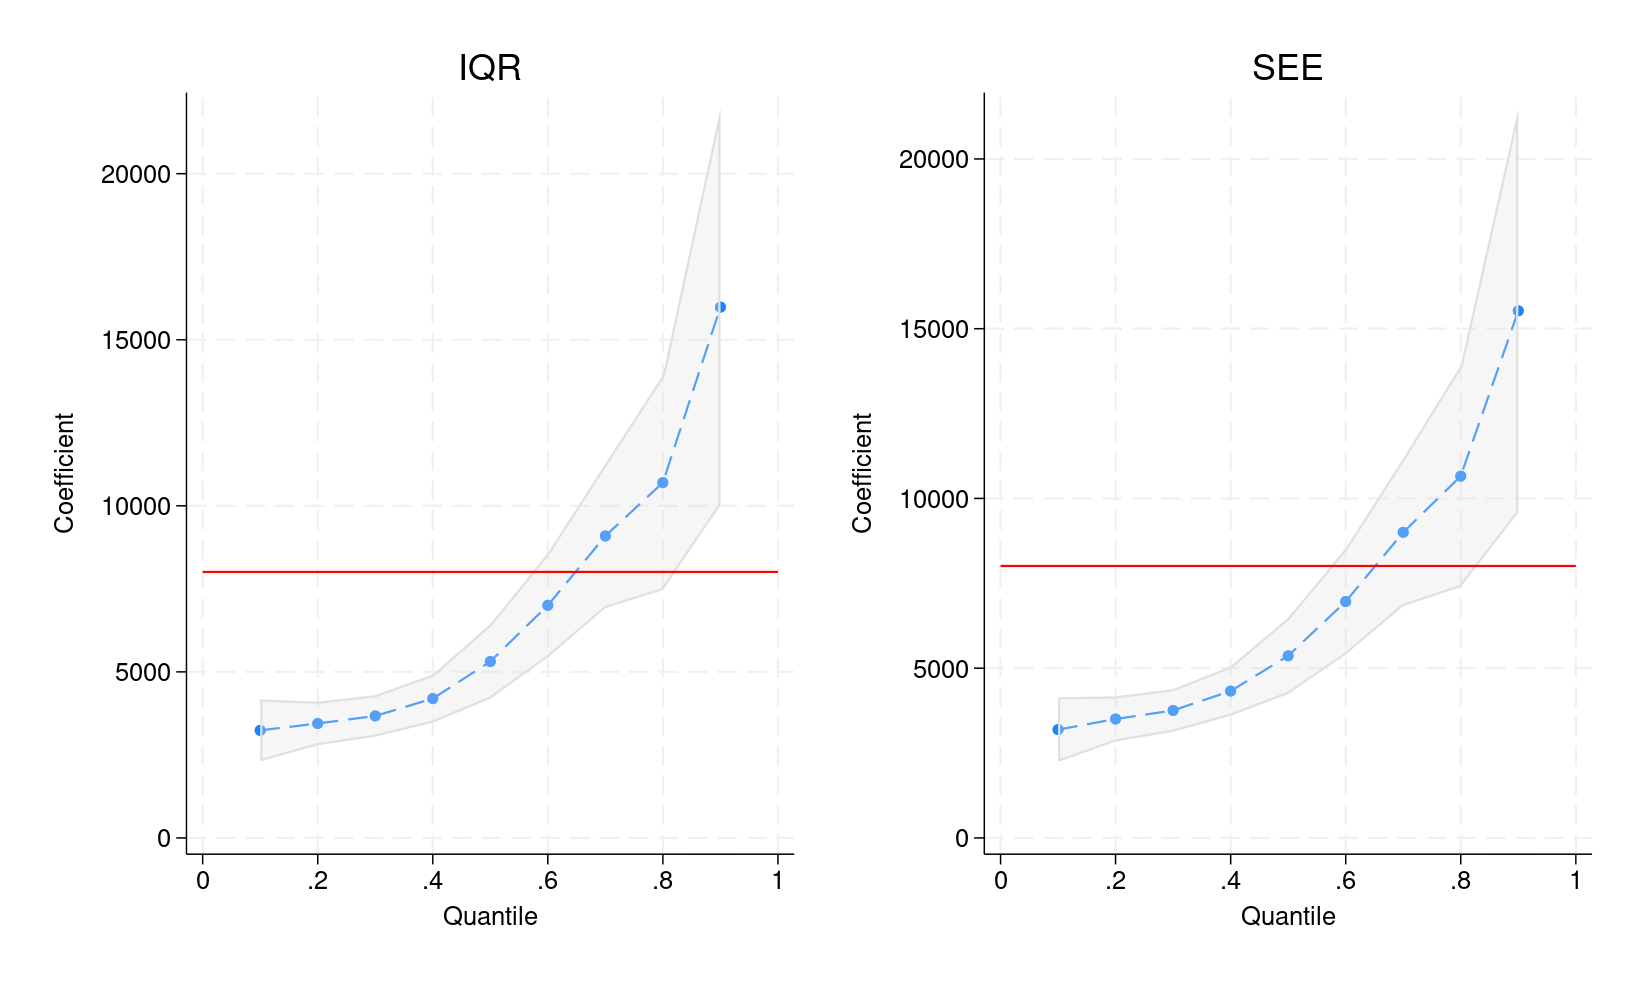
\includegraphics[scale=0.17]{eps/coefplot2}
\end{center}
\end{frame}

%------------------------------------------------------------------------------
\begin{frame}
  \frametitle{{\tt estat endogeffects}}
%------------------------------------------------------------------------------
  \stlogscaled{0.8}{./logs/ex1_e}
\end{frame}


%------------------------------------------------------------------------------
\section{Intuition and Simulations}
\begin{frame}
  \frametitle{IVQR model key moment condition}
%------------------------------------------------------------------------------
  \begin{align*}
    Pr&(y \leq \db'\alphab(\tau)  + \xb'\betab(\tau)|\myblue{\xb, \zb}) 
    = \tau
    \\
    & \hskip 3cm \Big\Downarrow  \\
    \E& \left[
      \left( \tau - \myred{\I(y - \db'\alphab(\tau)  - \xb'\betab(\tau) \leq 0)}
      \right)
    \myblue{\Psi(\xb, \zb)} \right]  = 0
  \end{align*}

  \begin{itemize}
    \setlength\itemsep{1em}
    \item The main \myred{difficulty} is the \myred{indicator} function $\I()$.
      The objective function is \myred{non-convex} and \myred{non-smooth}.

    \item In practice, \myblue{$\Psi(\xb, \zb) = (\Phi(\xb, \zb)', \xb')'$}, and
      \myblue{$\Phi(\xb, \zb)$ is the linear projection of $\db$ on the space
      spanned by $\xb$ and $\zb$}.

    \item $\Phi(\xb, \zb)$ can be regarded as transformed instruments for $\db$,
      so the over-identification can always be transformed into
      just-identification.
  \end{itemize}
\end{frame}

%------------------------------------------------------------------------------
\begin{frame}
\frametitle{Nonconvex and non-smooth objective function}
%------------------------------------------------------------------------------
\begin{figure}
\centering
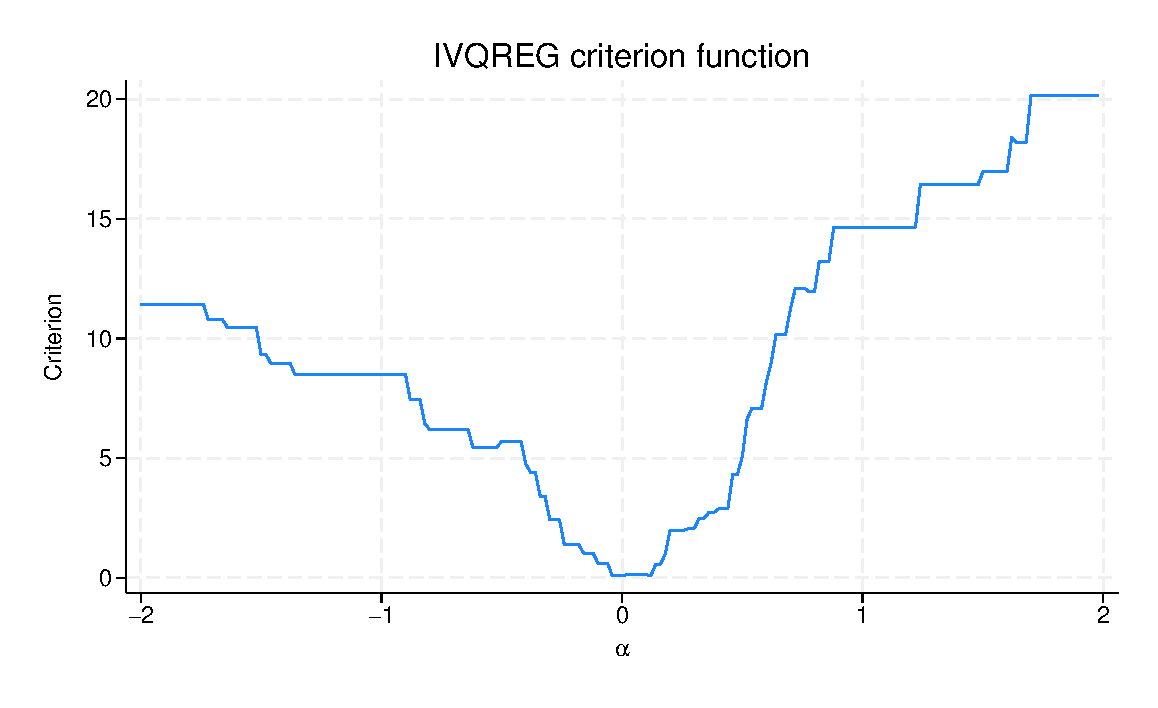
\includegraphics[scale=0.6]{eps/ivqreg_obj}
\caption{IVQREG GMM criterion function}
\end{figure}
\end{frame}

%------------------------------------------------------------------------------
\begin{frame}
  \frametitle{Intuition behind IQR and Smooth estimators}
%------------------------------------------------------------------------------

  \begin{itemize}
    \item {\bf IQR} (\citeauthor{chernozhukov2006}, 2006 and 2008)
    \setlength\itemsep{0.8em}

      \begin{itemize}
    \setlength\itemsep{0.5em}
	\item \myblue{Reduce} the \myblue{$p = dim(\alphab) + dim(\betab)$}
	  dimensional non-convex problem into \myblue{one-dimensional}
	  non-convex problem.

	\item Do a exhaustive grid search (in one dimension) over
	  \myblue{high quality of grid points}.
	
	\item The bounds for grid points are guarenteed to \myblue{cover the
	  true value with $95\%$ probability}.
	
	\item Good for \myred{only one endogenous variable}, but can compute the
	  \myblue{CI that is robust to the weak instrument}.
      \end{itemize}

    \item {\bf Smooth} \citep{kaplan2017}
      \begin{itemize}
    \setlength\itemsep{0.5em}
    \item \myblue{Smooth} the indicator function by \myblue{kernel} method.
    \item \myblue{Solve} a system of non-convex equation using 
      \myblue{\tt solvenl()}.
    \item Good for \myblue{more than one endogenous variables}, but \myred{can
      not provide the CI robust to weak instrument}.
  \end{itemize}
  \end{itemize}
\end{frame}

%------------------------------------------------------------------------------
\begin{frame}
  \frametitle{Simulation: DGP}
%------------------------------------------------------------------------------
  \begin{align*}
     y = \db' \alphab(u) + \xb' \betab(u) 	\\
     \myred{\alphab(\tau) = \betab(\tau) = 1 + \tau}
  \end{align*}
  \begin{itemize}
    \item $u$ is uniformly distributed.
    \item $\db$ is a linear function of instrument $\zb$ and it is correlated
      with $u$.
    \item $\xb$ is exogenous.
    \item When $dim(\db) = 1$, $dim(\zb) =$ 1, 2 or 3, $N = 1000$. Run {\tt
      qreg}, IQR, and Smooth.
    \item When $dim(\db) = 2$, $dim(\zb) =$ 2, 4, or 6, $N = 5000$. Run {\tt
      qreg} and Smooth.
    \item Estimate coefficients when $\tau = 0.1, 0.2, \ldots, 0.9$.
    \item The number of repetitions is $2030$.
  \end{itemize}
\end{frame}

%------------------------------------------------------------------------------
\begin{frame}
  \frametitle{Simulation: dim($\db$) = 1 (mean of $\hat{\beta}$)}
%------------------------------------------------------------------------------
  \begin{center} 
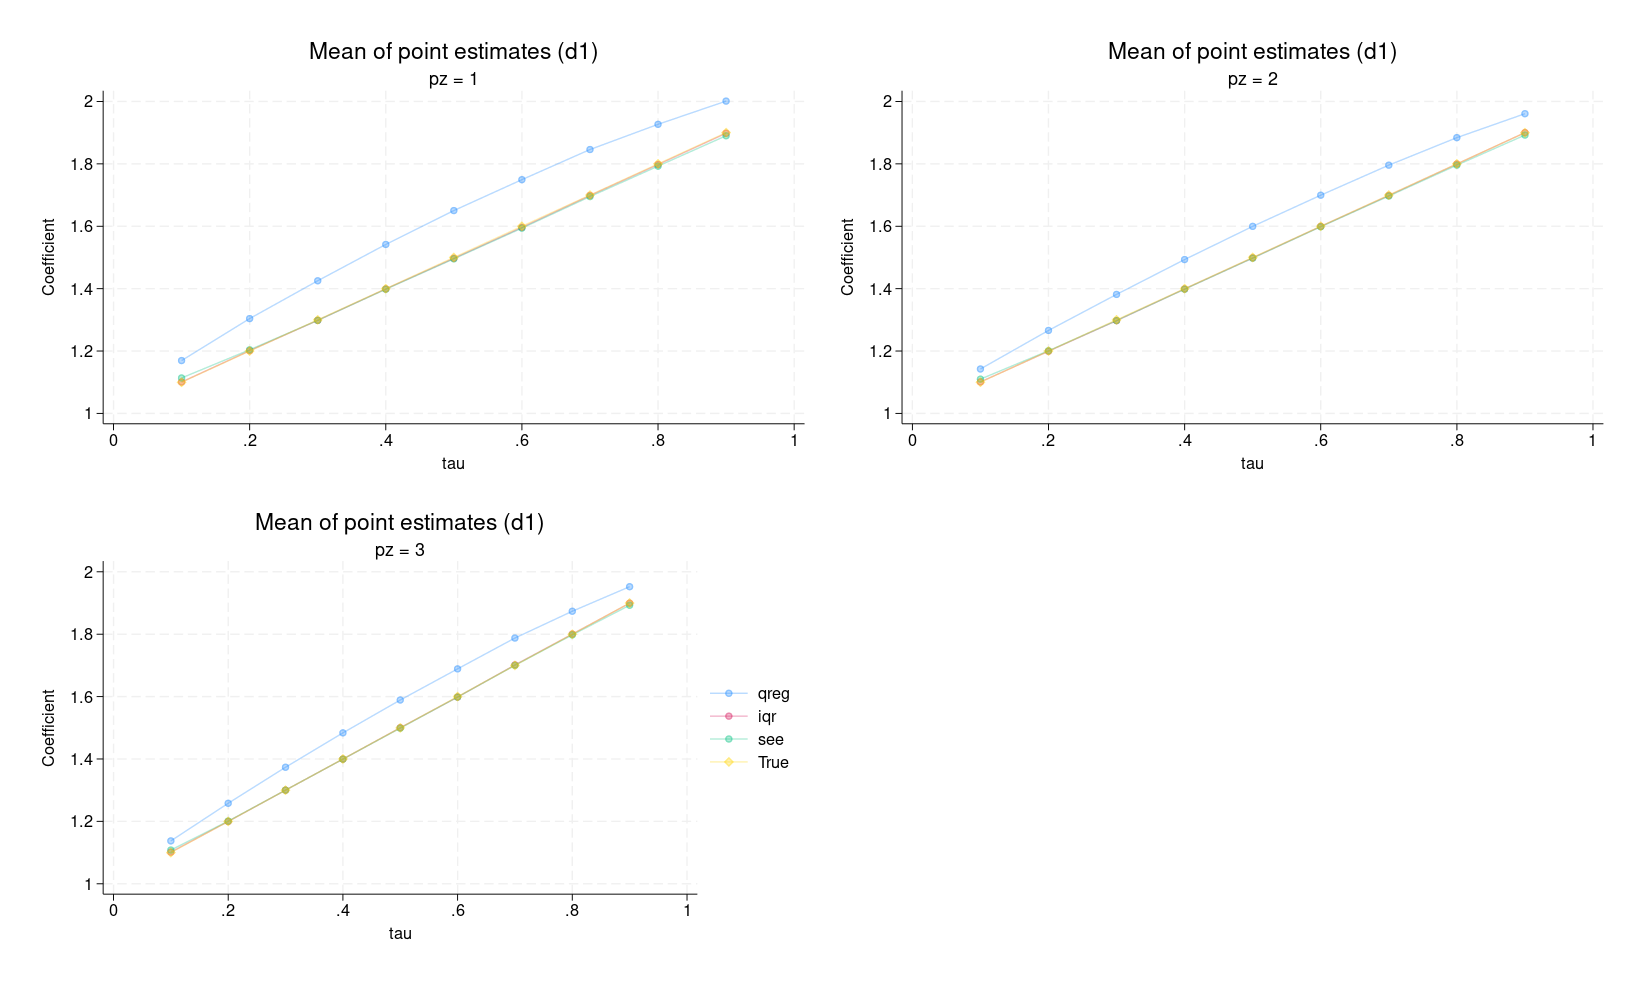
\includegraphics[scale=0.2]{eps/mbeta_d1}
\end{center}
\end{frame}

%------------------------------------------------------------------------------
\begin{frame}
  \frametitle{Simulation: dim($\db$) = 1 (bias)}
%------------------------------------------------------------------------------
  \begin{center} 
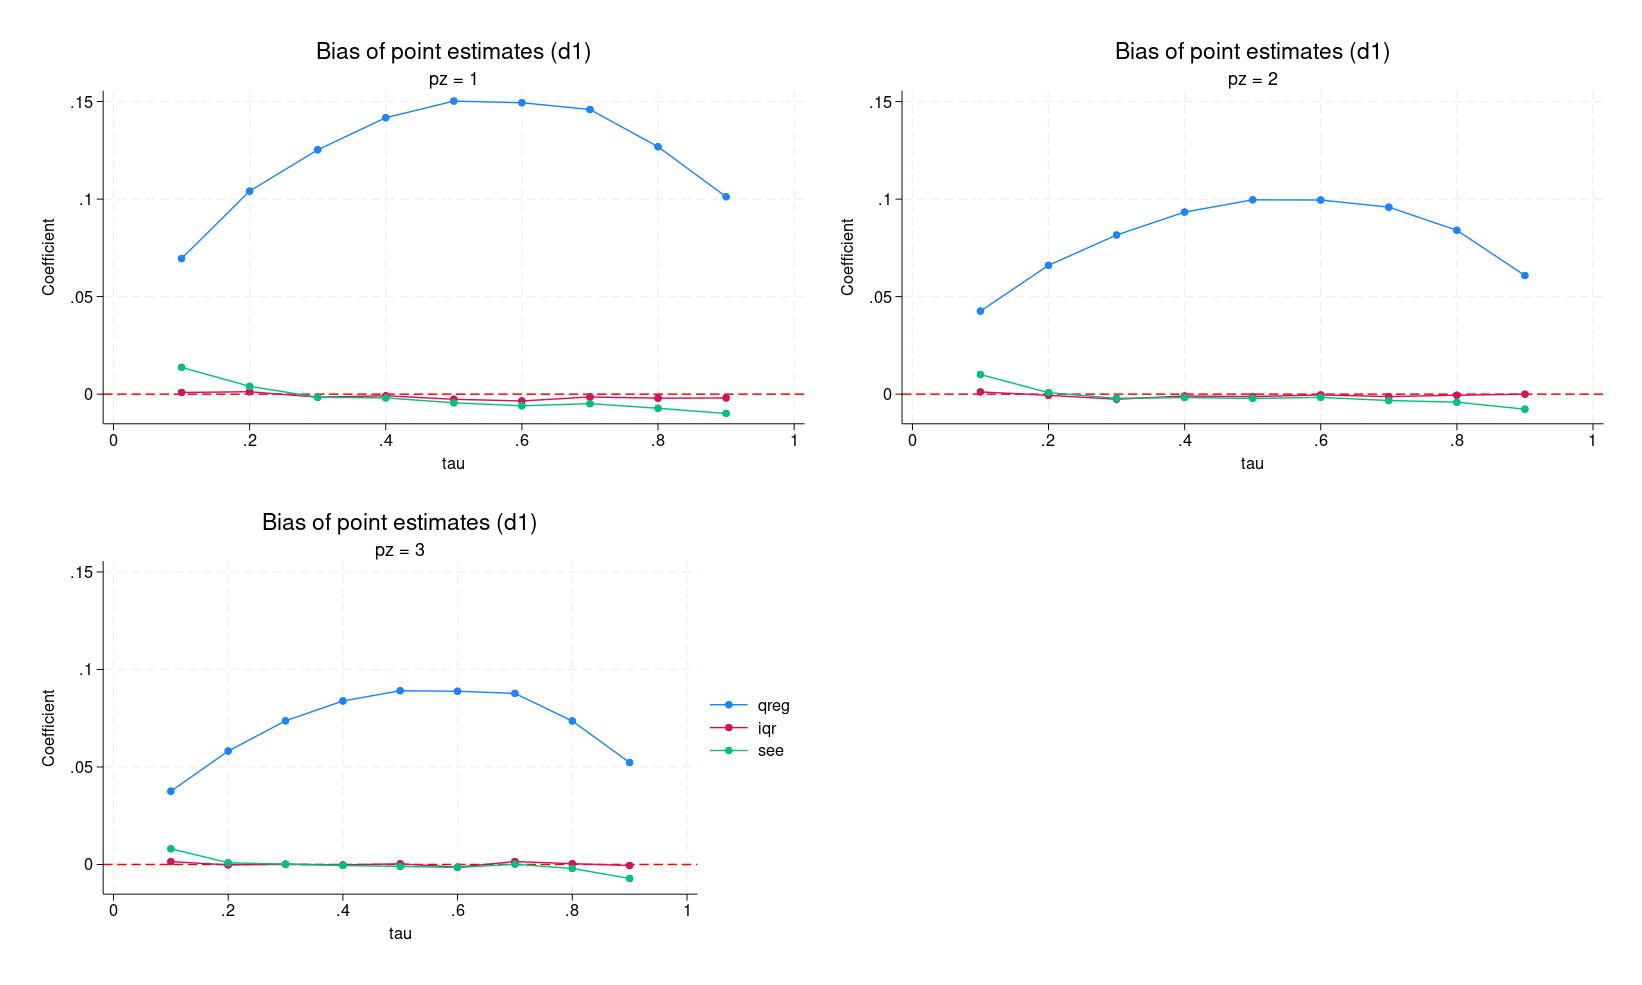
\includegraphics[scale=0.2]{eps/mbias_d1}
\end{center}
\end{frame}

%------------------------------------------------------------------------------
\begin{frame}
  \frametitle{Simulation: dim($\db$) = 1 (rejection rate)}
%------------------------------------------------------------------------------
  \begin{center} 
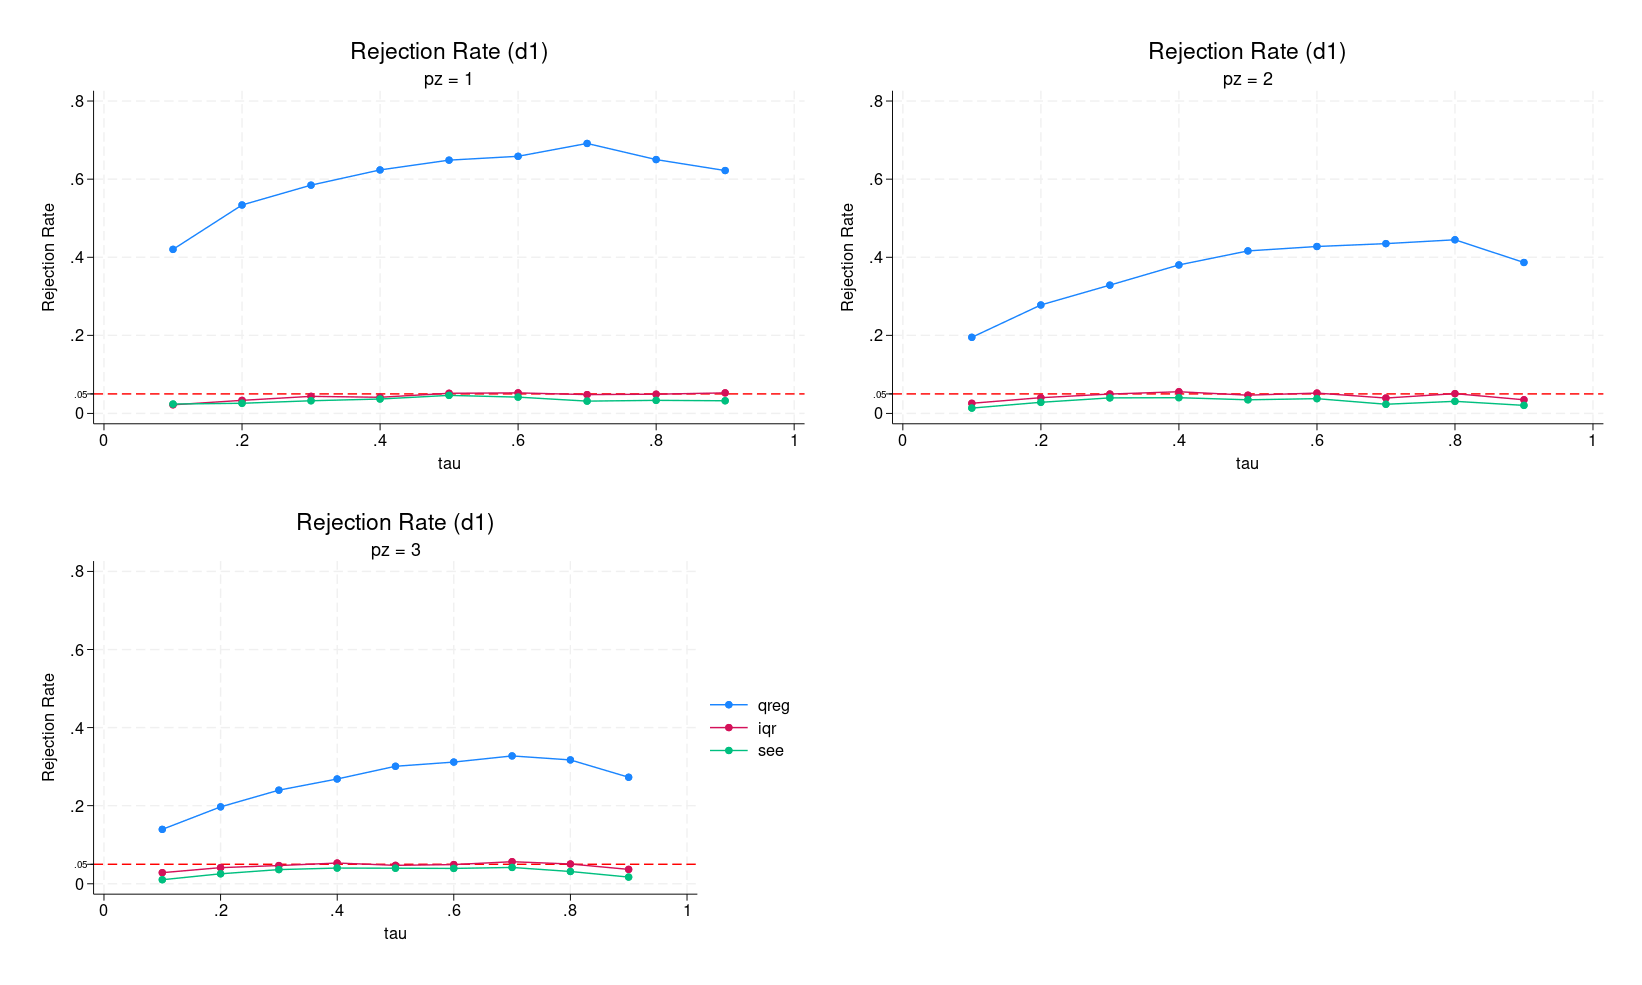
\includegraphics[scale=0.2]{eps/rej_d1}
\end{center}
\end{frame}

%------------------------------------------------------------------------------
\begin{frame}
  \frametitle{Simulation: dim($\db$) = 2 (mean of $\hat{\beta}$)}
%------------------------------------------------------------------------------
  \begin{center} 
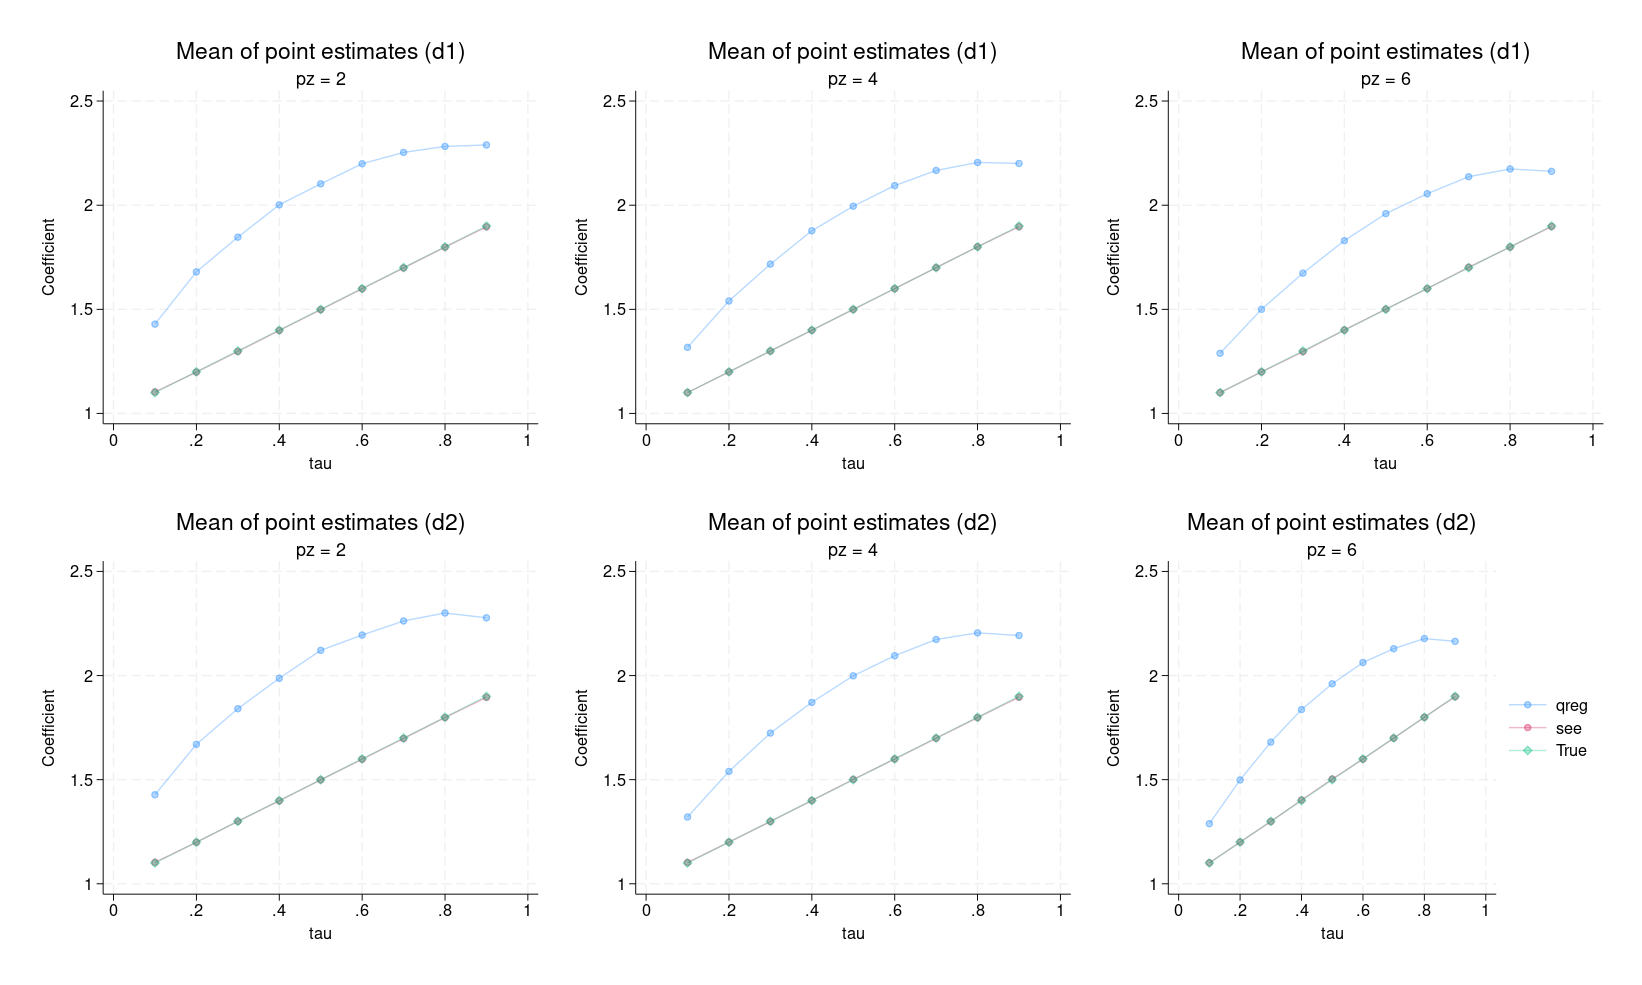
\includegraphics[scale=0.2]{eps/mbeta_d2}
\end{center}
\end{frame}

%------------------------------------------------------------------------------
\begin{frame}
  \frametitle{Simulation: dim($\db$) = 2 (bias)}
%------------------------------------------------------------------------------
  \begin{center} 
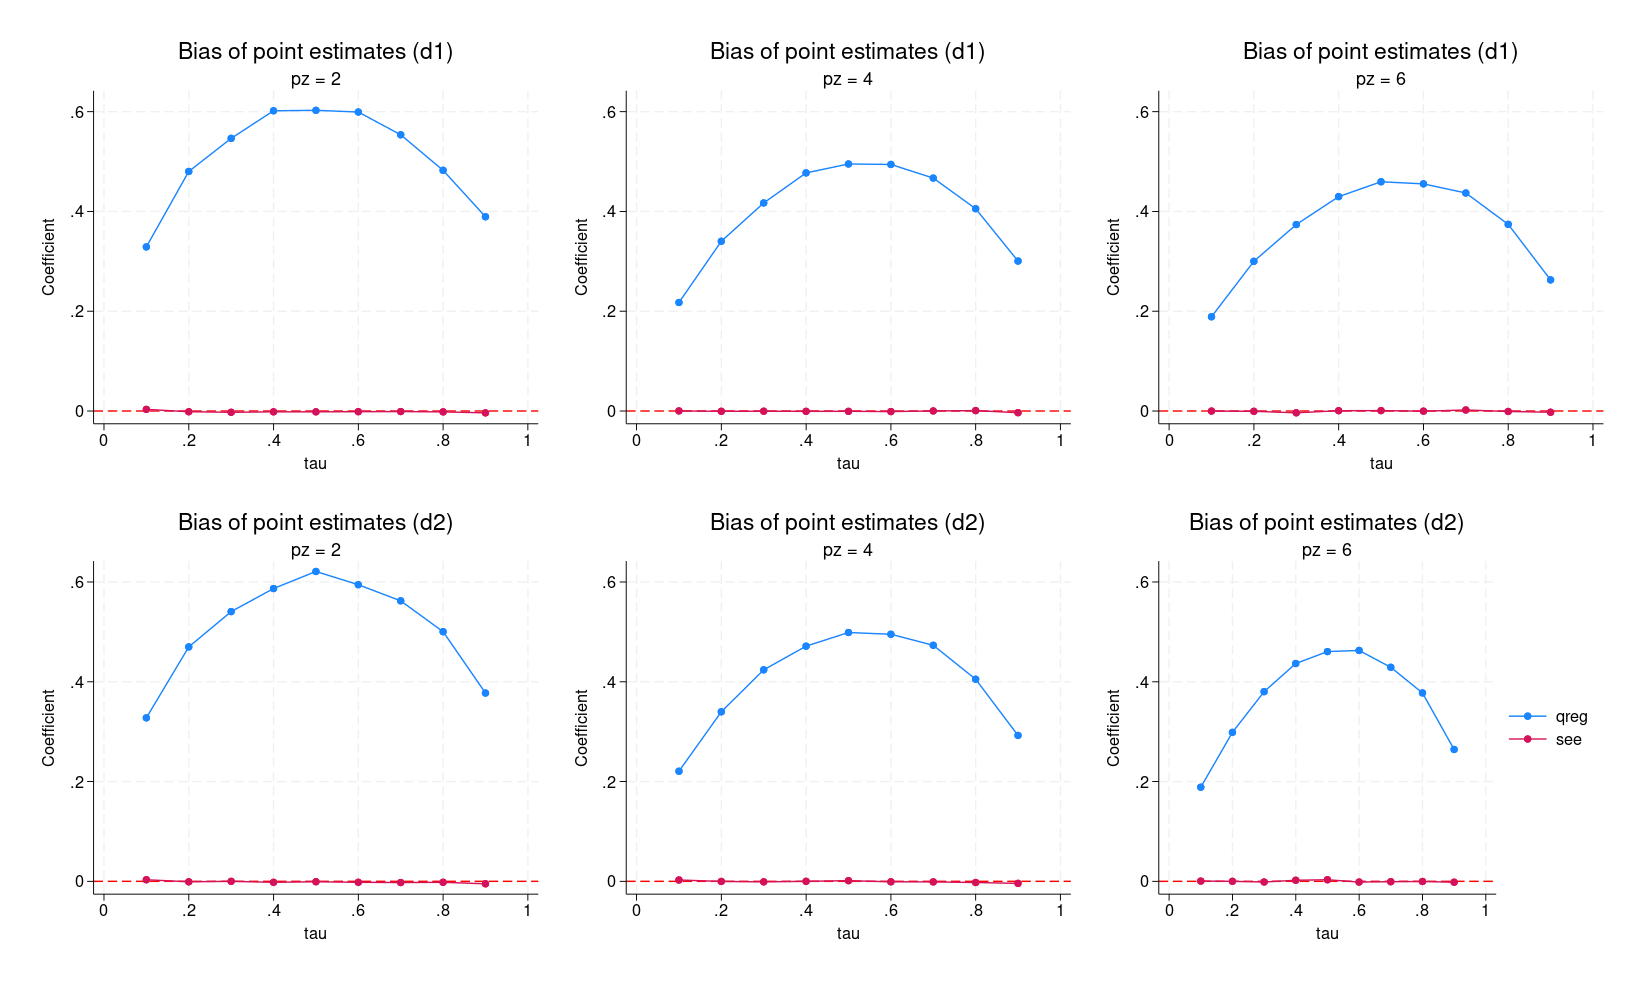
\includegraphics[scale=0.2]{eps/mbias_d2}
\end{center}
\end{frame}

%------------------------------------------------------------------------------
\begin{frame}
  \frametitle{Simulation: dim($\db$) = 2 (rejection rate)}
%------------------------------------------------------------------------------
  \begin{center} 
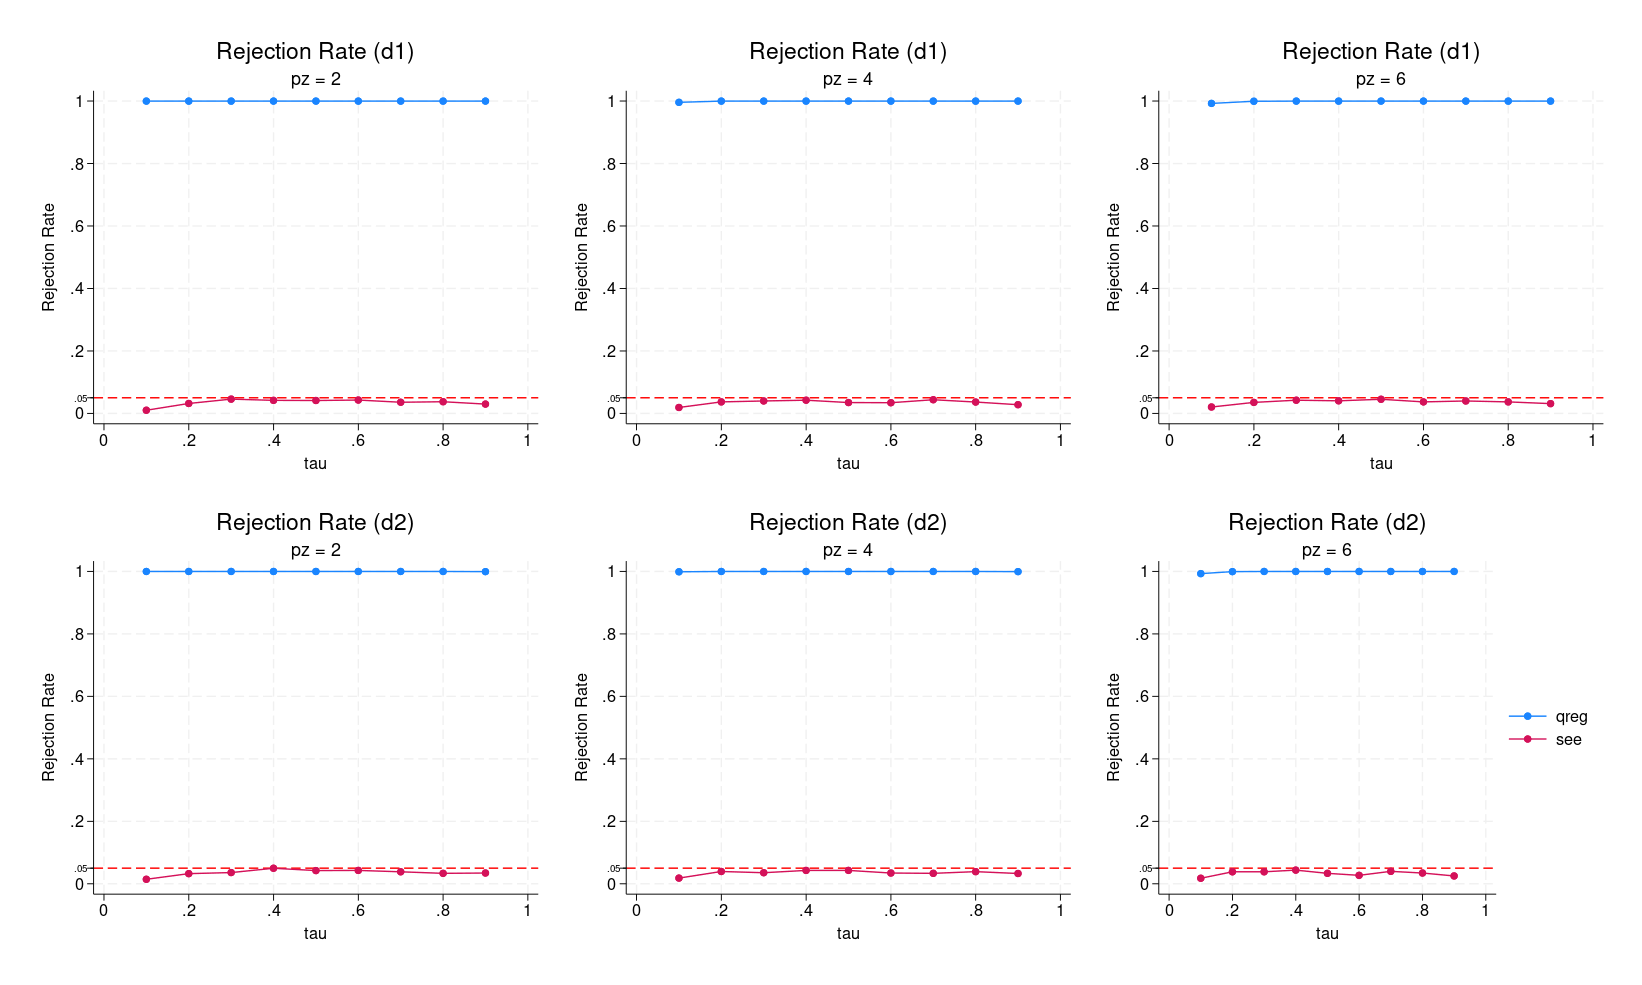
\includegraphics[scale=0.2]{eps/rej_d2}
\end{center}
\end{frame}






%------------------------------------------------------------------------------
\section{IQR Estimator}
\begin{frame}
  \frametitle{\myred{Inverse} quantile regression}
%------------------------------------------------------------------------------
  \begin{columns}

    \begin{column}{0.4\textwidth}
      \begin{center}
      \myblue{QREG}

      \big\Downarrow
      $$
      Pr( y \le \myblue{\zb}'\gamma(\tau) +
      \myblue{\xb}'\betab(\tau)|\myblue{\xb, \zb}) = \tau
	$$
      \big\Downarrow
      $$
	\min \sum_{i=1}^N \rho_{\tau}(y_i - \zb_i'\gamma - \xb_i'\beta)
	$$
      \Big\Downarrow

      {\tt qreg y x z}
  \end{center}
    \end{column}

    \begin{column}{0.6\textwidth}
      \begin{center}
      \myred{IVQREG}

      \big\Downarrow
      $$
	Pr( y \le \myred{\db'\alphab(\tau)} + \myblue{\xb'}\betab(\tau)
	|\myblue{\xb, \zb}) = \tau
	$$
	\big\Updownarrow
	$$
	Pr( y - \myred{\db'\alphab(\tau)}\le  \myblue{\xb'}\betab(\tau) +
	\myblue{\zb'*0}|\myblue{\xb, \zb}) = \tau
	$$
	\Big\Downarrow 

      {\tt qreg y-$\db'\alpha(\tau)$ x z}
  \end{center}
    \end{column}
  \end{columns}

  \vskip 0.5cm
  {\bf IQR} finds $\alpha(\tau)$ such that \myred{the coefficient on $\zb$ is as
  close to zero as possible}.
\end{frame}

%------------------------------------------------------------------------------
\begin{frame}
  \frametitle{Constructing grid using dual CI}
%------------------------------------------------------------------------------

\begin{itemize}
    \setlength\itemsep{1em}
  \item Given a grid of $A = \{\alpha_1, \ldots, \alpha_J\}$, {\bf IQR} finds
    $\alpha(\tau)$ such that \myred{the coefficient on $\zb$ is as close to zero
    as possible}, which is measured by the \myred{Wald statistic}
    ($W_n(\alphab(\tau))$).
  
  \item The grid points boundary must be \myblue{more comprehensive than the
    dual CI}, otherwise {\tt ivqregress iqr} will error out.

  \item Dual CI means it \myblue{covers the true value of $\alpha(\tau)$ with
    $95\%$} probability \citep{chernozhukov2008}.
\end{itemize}
\end{frame}

%------------------------------------------------------------------------------
\begin{frame}
  \frametitle{Dual CI}
%------------------------------------------------------------------------------
  \begin{prop}(Proposition 1 in
    \citeauthor{chernozhukov2008}[\citeyear{chernozhukov2008}])
When $\alphab =  \alphab(\tau)$,
\begin{align*}
  W_n[\alphab(\tau)] \rightarrow_d \chi^2(dim(\gammab))
\end{align*}
and for the confidence region $CR_p[\alphab(\tau)] = \{\alphab \in A:
W_n(\alphab) < c_p\}$, where $P(\chi^2(dim(\gammab)) < c_p) = p$,
\begin{align}
 \myred{ P\{\alphab(\tau) \in CR_p[\alphab(\tau)]\} = P\{ W_n[\alphab(\tau)] <
 c_p\} = p}
\end{align}
\end{prop}

\vskip 1cm
\myblue{$CR_p[\alphab(\tau)] = \{\alphab \in A: W_n(\alphab) < c_p\}$
covers the true value of $\alphab$ with probability approaching $p$}.
\end{frame}

%------------------------------------------------------------------------------
\begin{frame}
  \frametitle{ {\tt estat waldplot}}
%------------------------------------------------------------------------------
  \begin{center} 
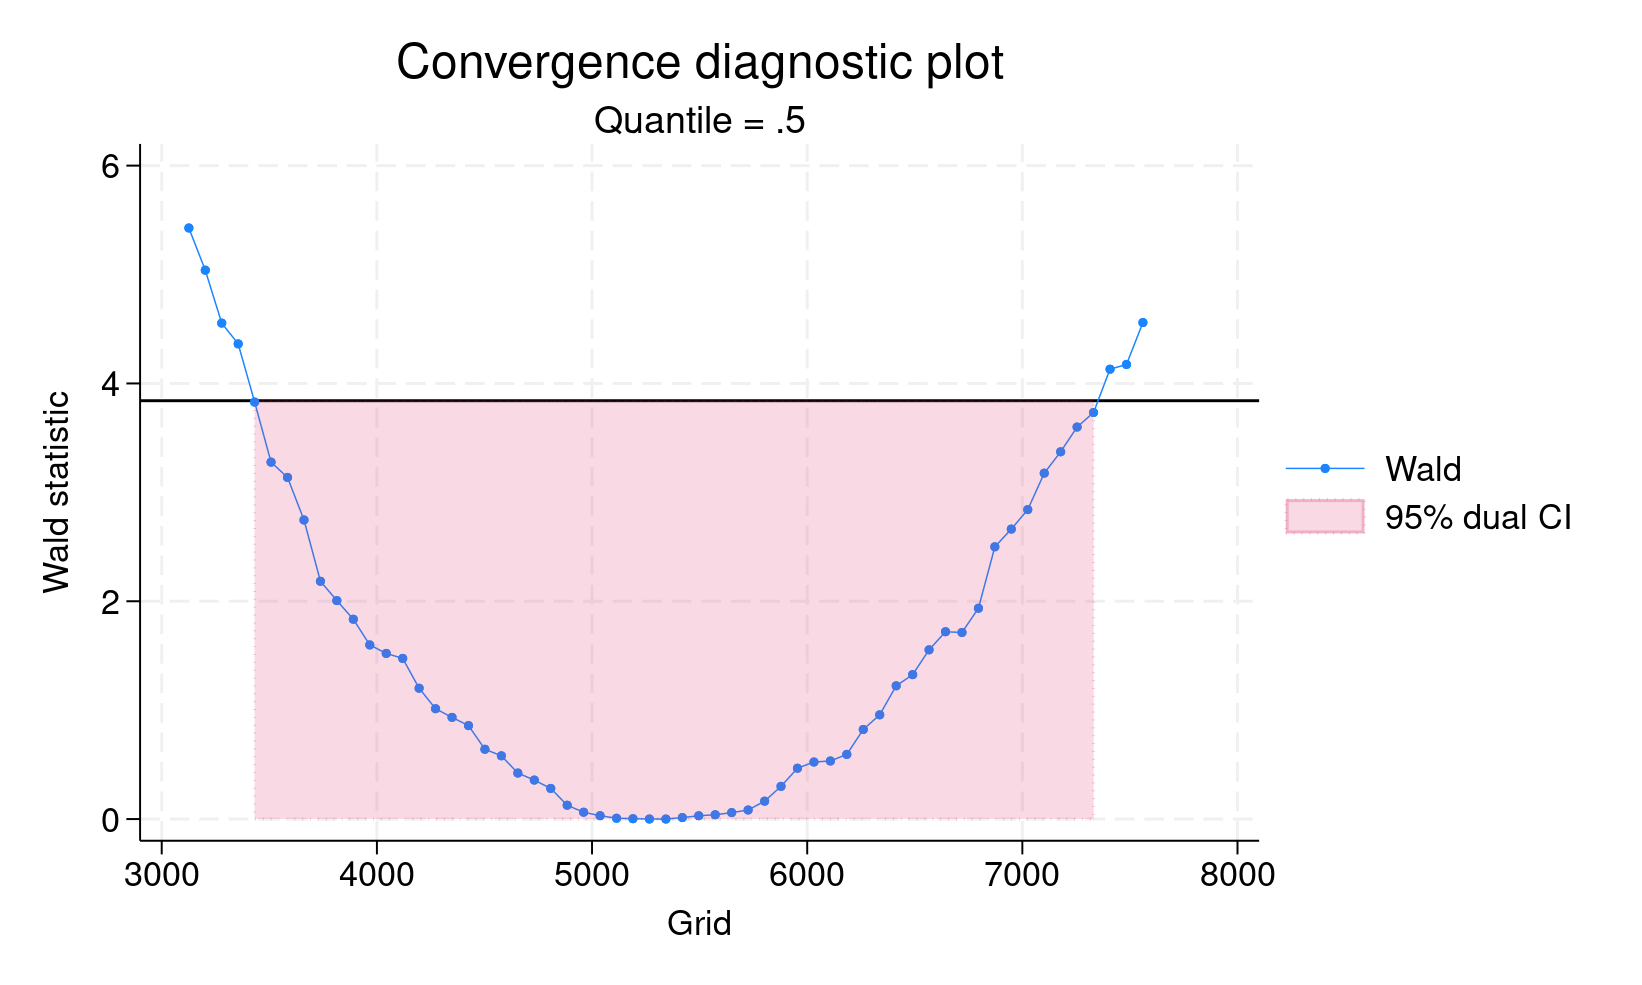
\includegraphics[scale=0.22]{eps/waldplot}
\end{center}
\end{frame}

%------------------------------------------------------------------------------
\begin{frame}
  \frametitle{ {\tt estat dualci}}
%------------------------------------------------------------------------------
\stlogscaled{0.87}{./logs/ex2_b}
\end{frame}

%------------------------------------------------------------------------------
\begin{frame}
  \frametitle{Simulation: Dual CI coverage with weak instruments}
%------------------------------------------------------------------------------
  \begin{center} 
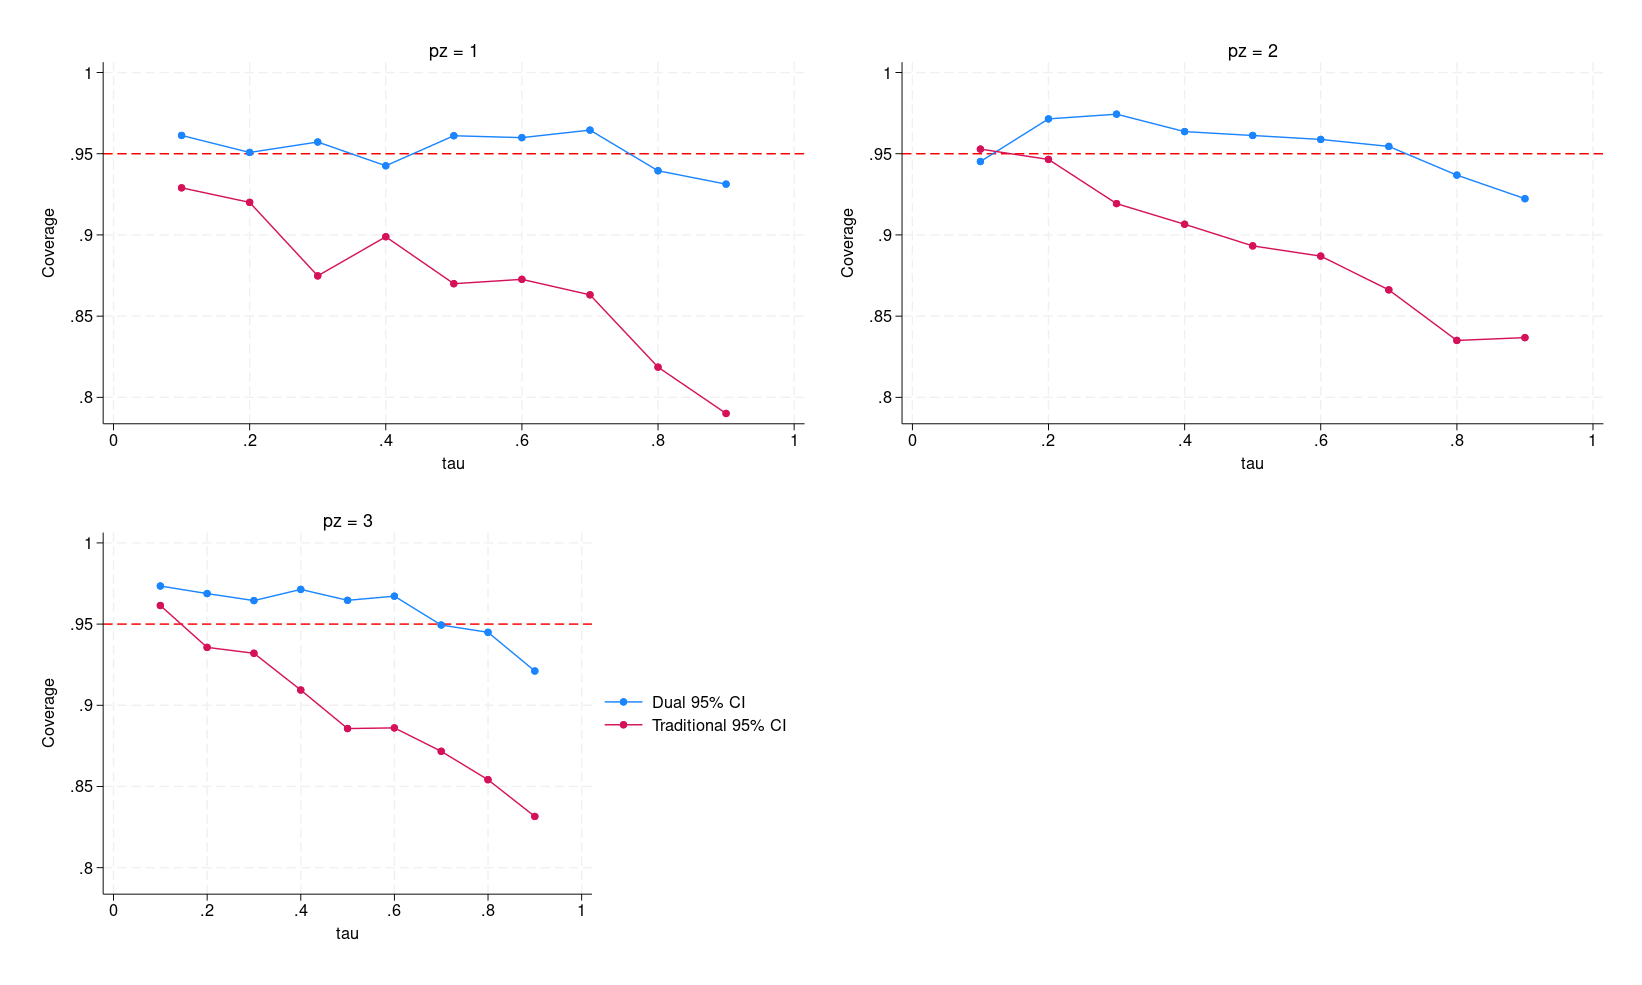
\includegraphics[scale=0.2]{eps/dualci}
\end{center}
\end{frame}

%------------------------------------------------------------------------------
\section{Smooth Estimator}
\begin{frame}
  \frametitle{Smoothed estimating equation estimator}
%------------------------------------------------------------------------------
  \begin{align*}
    \E \left[
      \left( \tau - \myred{\I\left(y - \db'\alphab(\tau)  -
      \xb'\betab(\tau)\right)}
      \leq 0)
      \right)
    \Psi(\xb, \zb) \right]  = 0 \\
    \Bigg\Downarrow \text{(smooth the indicator function by kernel)} \\
    \E \left[
      \left( \tau - \myblue{\widetilde{\I}\left(\frac{y - \db'\alphab(\tau)  -
      \xb'\betab(\tau)}{h}\right)}
      \leq 0)
      \right)
    \Psi(\xb, \zb) \right]  = 0 \\
  \end{align*}

  \begin{itemize}
    \item Solve this system of non-linear equation by {\tt solvenl()}. 

    \item The Smooth estimator is first-order equivalent to the IQR estimator so
      that we can use the same variance-covariance estimator
      \citep{DeCastro2019}.
   \end{itemize}
  
\end{frame}

%------------------------------------------------------------------------------
\begin{frame}
  \frametitle{Smoothed indicator function}
%------------------------------------------------------------------------------
  \begin{columns}
    \begin{column}{0.4\textwidth}
\begin{align*}
\Is(v) & =
\begin{cases}
  1 & \text{if $v \leq -1$} \\
  0 & \text{if $v \geq 1$}\\
  \frac{1-v}{2} &\text{if $-1 < v < 1$}
\end{cases}
\end{align*}
\end{column}

\begin{column}{0.6\textwidth}
\begin{center}
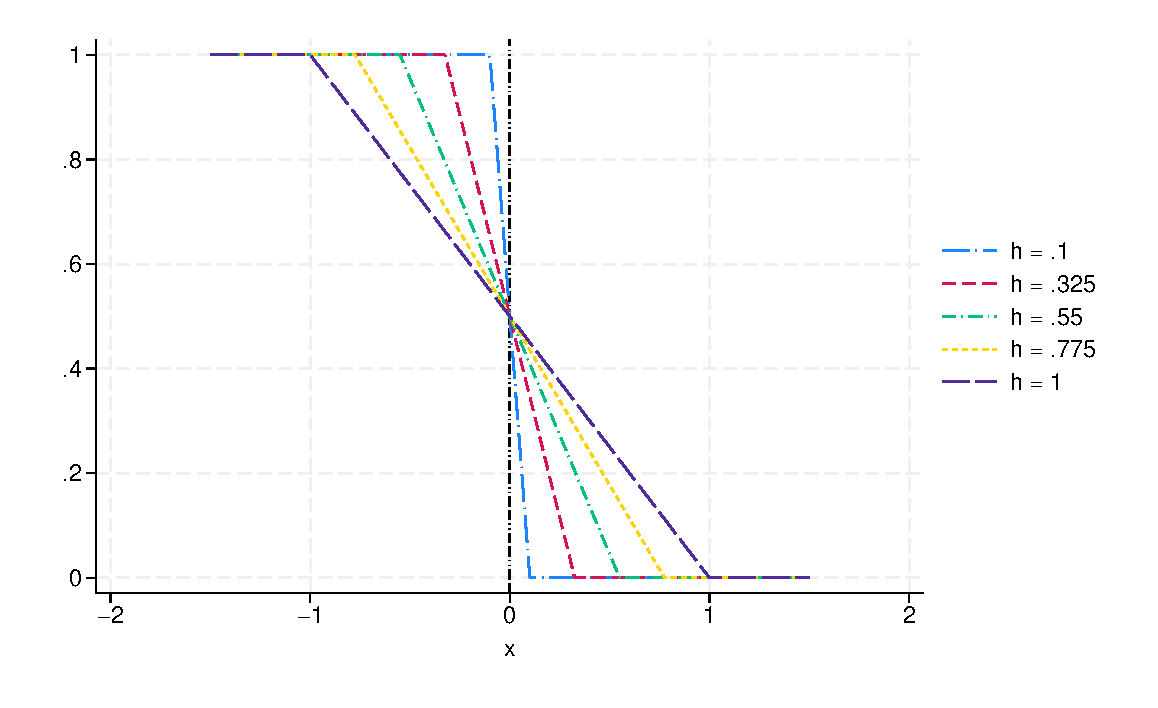
\includegraphics[scale=0.4]{eps/i_sgmm}
\end{center}
\end{column}
\end{columns}

\begin{itemize}
  \item The optimal bandwidth $h^*$ is chosen to minimize the MSE of the
    estimating equation.
  \item {\tt ivqregress} also requires that $h^*$ result in a $\alpha(\tau)$
    within the dual CI.
\end{itemize}
\end{frame}

%------------------------------------------------------------------------------
\section{Summary}
\begin{frame}
  \frametitle{Syntax of \ivqreg}
%------------------------------------------------------------------------------
{\scriptsize
\noindent
  \myred{I}nverse \myred{Q}uantile \myred{R}egression estimator:
\vskip 0.5cm


\begin{tabular}{ll}
  {\tt ivqregress \myred{iqr}} &{\it depvar } {\it $varlist_1$ }  
	({\it $varlist_2 = varlist_{iv}$}) [{\tt if}] [{\tt in}] 
	\hskip 0.1cm
	[ , {\it options} \hskip 0.1cm
	{\it IQR\_options} ]
\end{tabular}

\vskip 0.5cm

\noindent
\myred{S}moothed \myred{E}stimating \myred{E}quation estimator:
\vskip 0.5cm

\begin{tabular}{ll}
 {\tt ivqregress \myred{smooth}} &{\it depvar } {\it $varlist_1$ }  
	({\it $varlist_2 = varlist_{iv}$}) [{\tt if}] [{\tt in}] 
	\hskip 0.1cm
	[ , {\it options} \hskip 0.1cm {\it smooth\_options} ]
\end{tabular}
}


\vskip 0.5cm
\noindent
where
\begin{itemize}
    \setlength\itemsep{1em}
\item {\it $varlist_1$} specifies the exogenous variables.
\item {\it $varlist_2$} specifies the endogenous variables.  Only one continuous
variable or one binary factor variable is allowed for the inverse quantile
regression estimator.
\item {\it $varlist_{iv}$} specifies the instrumental variables.
\end{itemize}
\end{frame}

%------------------------------------------------------------------------------
\begin{frame}
  \frametitle{Post-estimation}
%------------------------------------------------------------------------------
The following postestimation commands are of particular interest after {\ivqreg}.

\vskip 0.5cm
{\footnotesize
\begin{tabular}{ll}
\hline
Commands & Description \\
\hline
{\tt estat coefplot} & plot coefficients and their confidence intervals \\
	& at different quantiles\\
{\tt estat endogeffects} & process test of no effect, constant effect,
stochastic \\
	& dominance, and endogeneity \\
*{\tt estat dualci} & provide the dual-confidence interval for 	
	the \\ &  endogenous variables \\
*{\tt estat waldplot} & plot Wald statistics corresponding to each grid point
\\
\hline
\end{tabular}

\vskip 0.5cm
Note :
\begin{itemize}
  \item {\tt estat waldplot} and {\tt estat dualci} are allowed only after {\tt
    ivqregress iqr}.
\end{itemize}
}

\end{frame}

%------------------------------------------------------------------------------
\begin{frame}
  \frametitle{Summary}
%------------------------------------------------------------------------------
  \begin{itemize}
    \setlength\itemsep{1em}

    \item We provide a suite of commands to estimate, visualize, and make the
      inference for the linear IVQR model.

    \item Two estimators: IQR and Smooth. Both are consistent, but the estimates
      may be different because they approximate the original estimating equation
      differently.

    \item IQR is widely used for the one endogenous variable case. It should be
      used as a benchmark because it provides the dual CI robust to the weak
      instrument.

    \item Smooth is suitable for the one or more endogenous variables case.

  \end{itemize}
\end{frame}


% reference
\clearpage
{\bf References}
\bibliographystyle{sjlatex/sj}
\bibliography{mybib}

{
\beamertemplatenavigationsymbolsempty
\setbeamercolor{background canvas}{bg=}
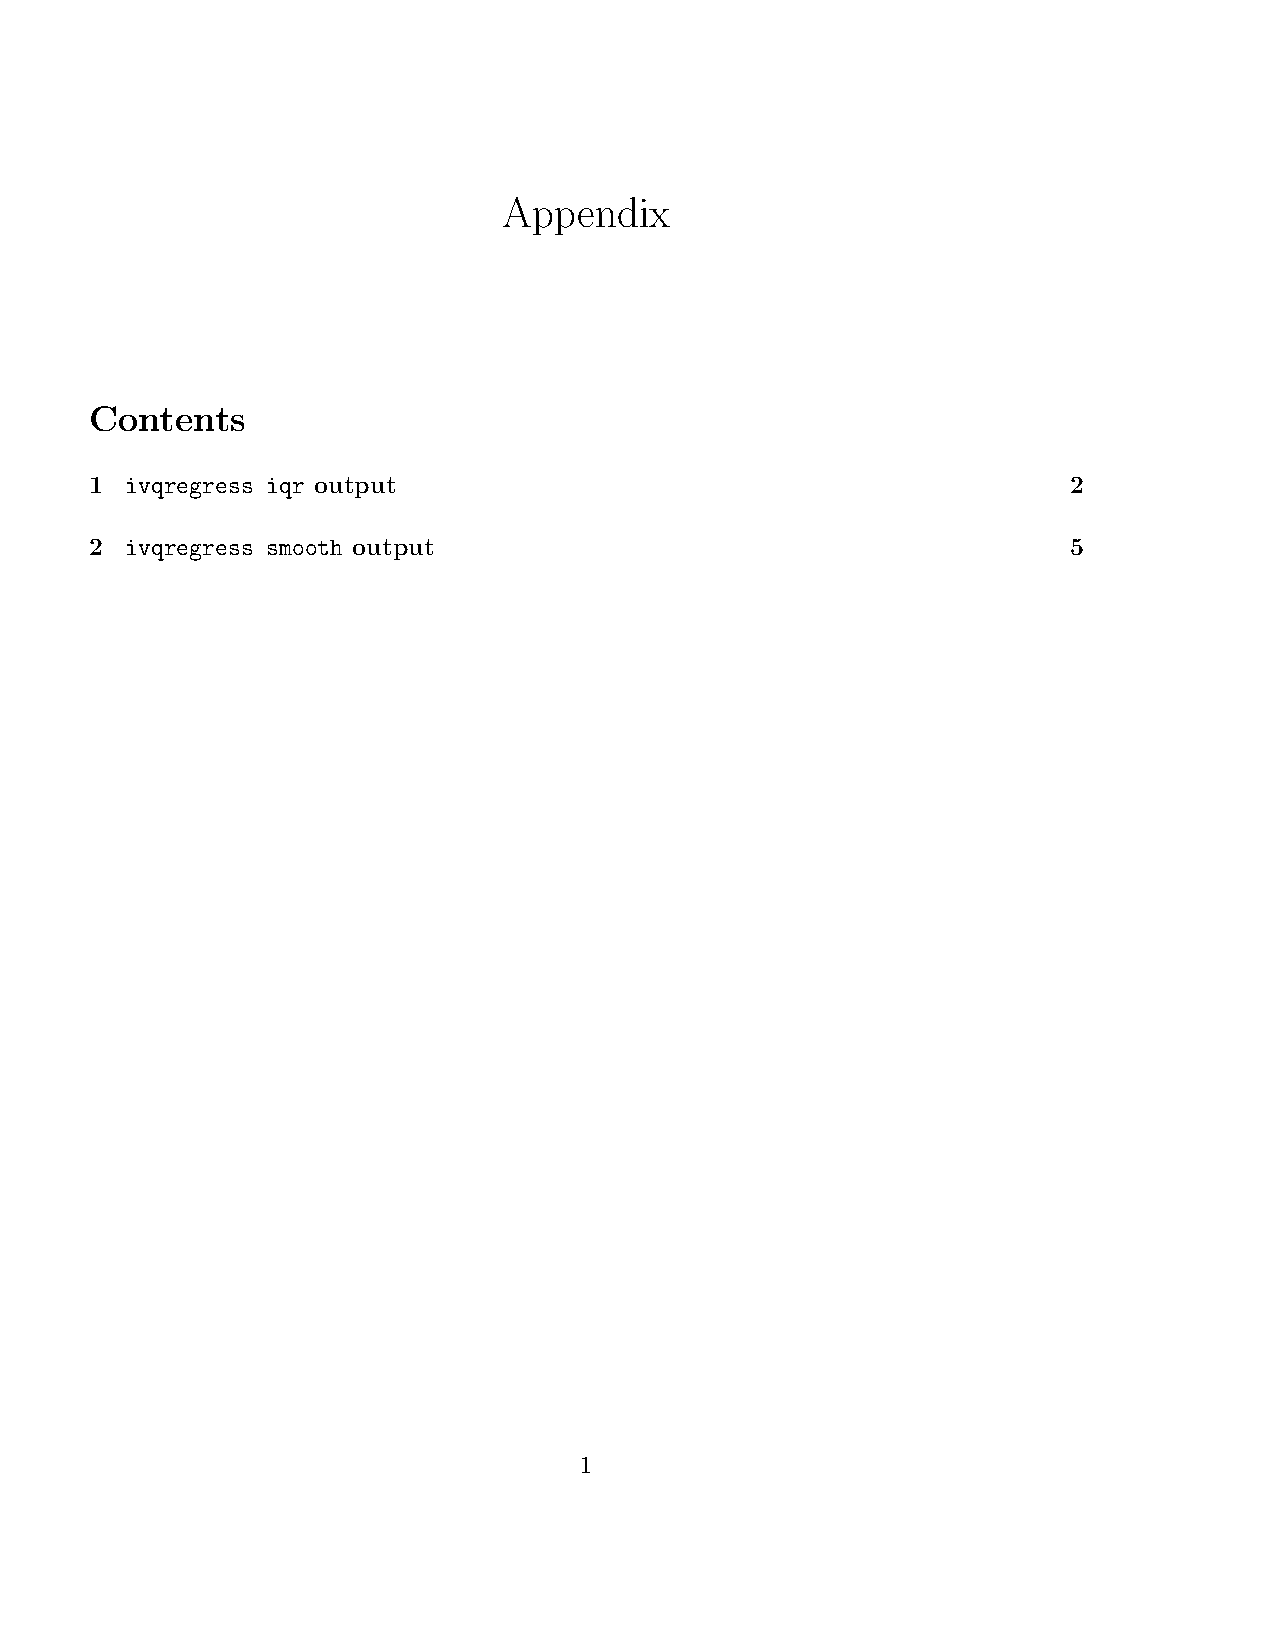
\includepdf[pages=1-9, link=true,fitpaper]{ivqreg_output.pdf}
}

\end{document}

